\section{Ejercicio 8 - Round Robin 2}

A continuación explicaremos nuestra implementación de un Scheduler Round Robin que no permite migración entre núcleos.

\subsection{Representación}

Para las tareas, hemos utilizado la misma estructura que en la implementación del scheduler Round Robin de la sección 4.

Para implementar el scheduler, hemos utilizado los siguientes atributos:

\begin{itemize}
\item la cantidad de cores
\item un arreglo de enteros de tamaño cantidad de cores utilizados, donde cada entero representa el quantum correspondiente a dicho core
\item un arreglo de enteros del mismo tamaño, donde cada entero representa la cantidad de tareas que están asignadas a diho core
\item un arreglo de tareas del mismo tamaño, donde cada tarea representa la tarea que actualmente está corriendo en dicho core
\item un arreglo del mismo tamaño conteniendo una lista de tareas en cada posición, donde cada lista contiene a las tareas en estado {\it ready} y {\it waiting} para cada core.
\end{itemize}

\subsection{Funciones}

\paragraph{Load} Se crea una nueva tarea con el pid indicado, se recorre el arreglo con la cantidad de tareas por cpu, y se agrega como último elemento de la lista de tareas correspondiente al cpu con menos tareas.

\paragraph{Unblock} Se recorre la lista de tareas {\it ready} y {\it waiting} de cada cpu hasta encontrar a la tarea con el pid indicado, y colocarla como ``no bloqueada''.

\paragraph{Tick} Se cuenta con tres casos:

\subparagraph{TICK} Primeramente se decrementa el quantum restante de la tarea actual en el cpu indicado.  Si aún tiene quantum para correr, se devuelve su pid.  En caso de que se haya terminado su quantum, se evaluará si existe otra tarea en estado {\it ready}.  De ser así, se devolverá el pid de la primer tarea que se encuentre en dicho estado en la lista de tareas correspondiente al cpu indicado.  Si no hay otra tarea para correr, sea porque todas las demás se encuentran bloqueadas o porque no existen más tareas, se devuelve el pid de la tarea actual del cpu indicado.
\subparagraph{BLOCK} Se coloca la tarea actual del cpu indicado como ``bloqueada'', se la coloca al final de la lista de tareas del cpu indicado y se procede a buscar la siguiente tarea a ejecutar.  Si no hay más tareas o todas están bloqueadas, se devuelve la constante IDLE_TASK.  En caso contrario, se devuelve el pid de la primer tarea en estado {\it ready} que se encuentre al recorrer la lista correspondiente.
\subparagraph{EXIT} En primer lugar, se decrementa la cantidad de tareas del cpu indicado. Si no hay más tareas o todas están bloqueadas, se devuelve la constante IDLE_TASK.  En caso contrario, se devuelve el pid de la primer tarea en estado {\it ready} que se encuentre al recorrer la lista.

\subsection{Migración vs No Migración}

La migración entre núcleos puede ser beneficiosa o no dependiendo del contexto de uso.  Por este motivo, mostraremos un escenario factible en el que la migración entre núcleos es conveniente y otro caso en el cual no lo es. Ambos casos serán planteados sin llamadas bloqueantes para una mejor comprensión.  Además, mostraremos cada escenario a través del simulador, considerando un cambio de contexto de 1 ciclo, 2 cores y un costo de migración de 4 ciclos.

En un caso en el cual se tienen algunas tareas que hacen un uso de CPU por un tiempo extenso y otras que lo utilizan durante poco tiempo, si no se utiliza migración entre núcleos podría ocurrir que las tareas extensas estén corriendo en un core y las demás en otro. La Figura \ref{fig-c2} muestra un ejemplo en el que ocurre esto, y podemos notar que el núcleo 1 rápidamente queda ocioso, mientras que el núcleo 0 sigue corriendo las tareas más pesadas. Por el contrario, la Figura \ref{fig-c1} muestra el mismo caso pero utilizando migración, y es evidente cómo se hace un mejor uso de ambos núcleos y, por lo tanto, el tiempo total de ejecución de las tareas más extensas se reduce considerablemente.  Si tomamos el tiempo total de ejecución de cada tarea en cada caso, obtenemos para la Figura \ref{fig-c2} un promedio de 54 ciclos, mientras que en la Figura \ref{fig-c1} tenemos un promedio de 32 ciclos.  Además, en el primer caso el núcleo 1 se mantuvo ocioso durante 78 ciclos, mientras que en el segundo sólo lo hizo durante 1 ciclo.

\begin{figure}[!htb]
\begin{center}
  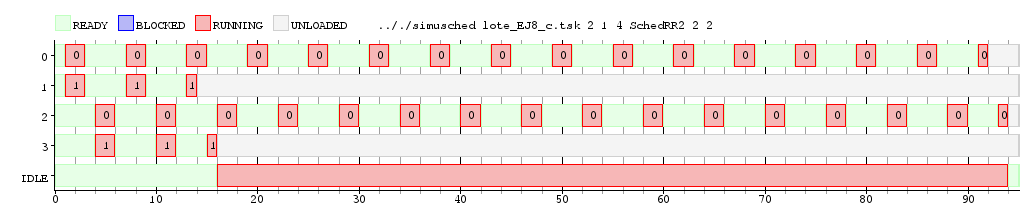
\includegraphics[scale=0.45]{imagenes/rr2-conviene.png}
\end{center}
\caption{No migración de núcleos no beneficiosa}\label{fig-c2}
\end{figure}

\begin{figure}[!htb]
\begin{center}
  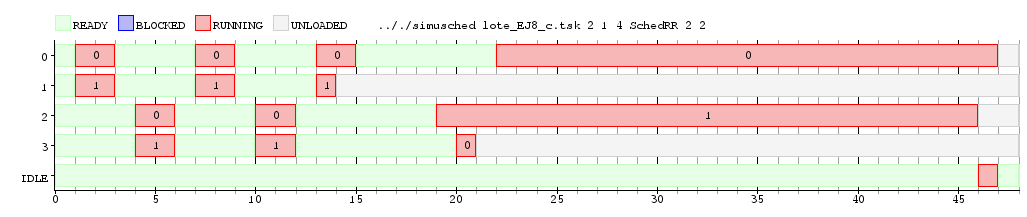
\includegraphics[scale=0.45]{imagenes/rr-conviene.png}
\end{center}
\caption{Migración de núcleos beneficiosa}\label{fig-c1}
\end{figure}

Otro caso que podría darse es que se pongan a ejecutar varias tareas cortas de manera secuencial.  Considerando que la migración entre núcleos suele ser bastante costosa, si se requieren numerosas migraciones hasta que cada tarea termina, el waiting-time de ellas se incrementaría de manera considerable, lo cual puede ser poco conveniente dado que se trata de tareas de corta duración.  Esto puede verse en la Figura \ref{fig-nc1}, mientras que, como muestra la Figura \ref{fig-nc2}, no migrar estos procesos permite que terminen en menor tiempo y, por lo tanto, disminuya su waiting-time.  Observando la Figura \ref{fig-nc1} podemos determinar un waiting-time promedio entre todas las tareas de 30,17, mientras que el mismo valor en la Figura \ref{fig-nc2} es de 14.

\begin{figure}[!htb]
\begin{center}
  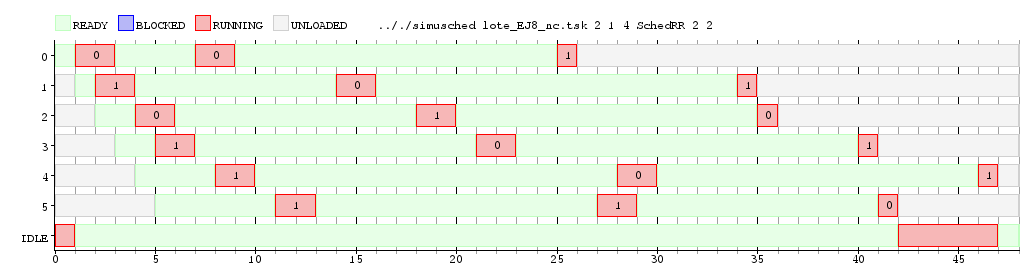
\includegraphics[scale=0.45]{imagenes/rr-noconviene.png}
\end{center}
\caption{Migración de núcleos no beneficiosa}\label{fig-nc1}
\end{figure}

\begin{figure}[!htb]
\begin{center}
  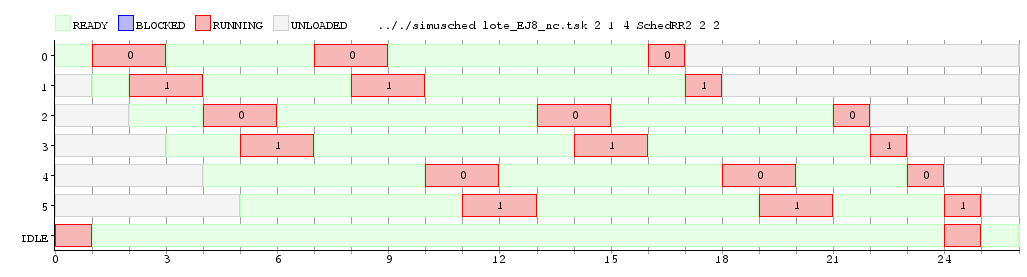
\includegraphics[scale=0.45]{imagenes/rr2-noconviene.png}
\end{center}
\caption{No migración de núcleos beneficiosa}\label{fig-nc2}
\end{figure}